% generated by src/r2/paper_assets (make_paper_assets.py figures); do not edit by hand
% provenance: figS7_recovery_calibration generated by src/r2/paper_assets on 2026-10-15 04:07 from data/r2/tables/
%   fit_recovery_calibration.csv (modified 2026-10-14 20:12): in_ece_bins1_9 == True (bins 1-9); all estimators; simulator = faithful_cc (design-faithful)
%   fit_recovery.csv (modified 2026-10-14 20:12): simulator = faithful_cc: analysis_status of the truth-start estimator and of quantity ece_bins1_9 (post hoc flags)
%   modes_faithful_design.csv (modified 2026-10-14 20:12): quantity = n_edges_cc_observed, sim_label in {immune_cc, global_cc}: ratio_sim_mean_to_real
\begin{figure}[htbp]
  \centering
  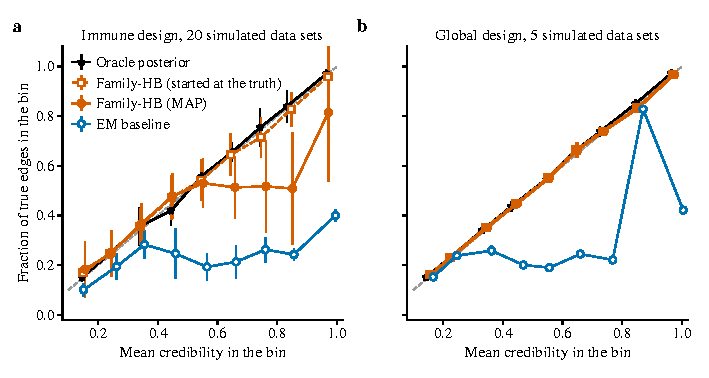
\includegraphics[width=0.75\textwidth]{figS7_recovery_calibration.pdf}
  \caption{\textbf{Calibration of credibility in simulation.} Data simulated from the fitted Family-HB model with the real literature observation masks and the motif/coexpression masks rebuilt from the simulated literature reports (design-faithful simulator; the simulated data contain 59\% (immune) and 62\% (global) of the real number of motif- or coexpression-observed edges). Edges are binned by credibility (bins from 0.1 to 1; the bin below 0.1, which holds almost all edges, is omitted); points: pooled fraction of truly regulatory edges against the mean credibility in the bin; bars: $\pm 1$ SD of that fraction across simulated data sets; dashed line: perfect calibration. Started at the true parameters, Family-HB is close to the oracle posterior; multi-start MAP selects the competing mode in some data sets (immune 2 of 20, global 0 of 5), which pulls the upper bins down and widens their spread; the EM baseline is over-confident (fraction of true edges more than 0.01 below the mean credibility) in 16 of its 18 universe $\times$ bin cells. The design-faithful simulation is post hoc (defined after the held-out data had been examined; it uses no held-out data).}
  \label{fig:S-recovery}
\end{figure}
